\section{Modeling }\label{sec:model}
%
% {\color{blue} EDITABLE}
%
% Section outline:
%
% \begin{enumerate}
% \item \cmark section intro
% \item \cmark fix order from simplest to most complex
% \item Description of DCE and parameter estimation
% \item\cmark Description of auto ARIMA
% \item \cmark Description of the two naive methods (random walk and mean), make sure to explain that these methods are naive and simple but not necessarily bad.
% \item\cmark Add a section talking about evaluation methods i.e., MASE, this text is currently written and just sitting at the beginning of the results.
%
% \end{enumerate}

In this section, we describe the four different forecasting methods
used in this study, as well as the error metric used to evaluate their
predictive accuracy.  These methods include:
\begin{itemize}
\item The \emph{random-walk} method, which uses the previous value in
  the observed signal as the forecast,

\item The \emph{\naive} method, which uses the mean of the
  observed signal as the forecast,

\item The \emph{ARIMA} (auto-regressive integrated moving average)
  method, a common linear forecast strategy, and

\item The \emph{LMA} (Lorenz method of analogues) method, which uses a
  near-neighbor forecast strategy on a dynamical reconstruction of the
  signal.
\end{itemize}
ARIMA is based on standard autoregressive techniques.  LMA is designed
to capture and exploit the deterministic structure of a signal from a
nonlinear dynamical system.  The \naive ~and random-walk methods,
somewhat surprisingly, often outperform these more-sophisticated
prediction strategies in the case of highly complex signals, as
discussed below.

\subsection{Two Simple Prediction Strategies}
\label{sec:simple}

A random-walk predictor simply uses the last observed measurement as
the forecast: that is, the predicted value $p_i$ at time $i$ is
calculated using the following relation: $$p_i = x_{i-1}$$ The
prediction strategy that we refer to using the term ``\naive''
averages the prior observations to generate the forecast: $$p_i =
\sum_{j=1}^{i-1}\frac{x_j}{i-1}$$ While both of these methods are
simplistic, they are not without merit.  For a time series near the
high end of the complexity spectrum---i.e., one that possesses very
little predictive structure---these two methods can actually be the
best choice.  In forecasting currency exchange rates, for instance,
sophisticated econometrics-based prediction models fail to
consistently outperform the random-walk method~\cite{rwMeese,rwCCE}.
These signals are constantly changing, noisy, and possess very little
predictive structure, but their variations are not---on the
average---very large, so the random-walk method's strategy of simply
guessing the last known value is not a bad choice.  If a signal has a
unimodal distribution with low variance, the \naive ~prediction
strategy will perform quite well---even if the signal is highly
complex---simply because the mean is a good approximation of the
future behavior.  Moreover, the \naive ~prediction strategy's temporal
average effects a low-pass filtering operation, which can  mitigate the
complexity in signals with very little predictive structure.

Both of these methods have significant weaknesses, however.  Because
they do not model the temporal patterns in the data, or even the
distribution of its values, they cannot track changes in that
structure.  This causes them to fail in a number of important
situations.  Random-walk strategies are a particularly bad choice for
time series that change significantly at every time step.  In the
worst case---a large-amplitude square wave whose period is equivalent
to twice the sample time---a random-walk prediction would be exactly
180 degrees out of phase with the true continuation.  The \naive
~method would be a better choice in this situation, since it would
always split the difference.  It would, however, perform poorly when a
signal has a number of long-lived regimes that have significantly
different means.  In this situation, the inertia of the \naive
~method's accumulating mean is a liability and the agility of the
random-walk method is an advantage, since it can respond quickly to
regime shifts.

Of course, methods that could capture and exploit the geometry of the
data, or its temporal patterns, would be far more effective in the
situations described in the previous paragraph.  The ARIMA and LMA
methods introduced in Sections~\ref{sec:arima} and~\ref{sec:lma} are
designed to do exactly that.
% Note, though, that periodic patterns
%appear only in signals that are at the low end of the %complexity
%spectrum.
However, if a signal contains little predictive structure, forecast
strategies like ARIMA and LMA have nothing to work with and thus will
often be outperformed by the two simple strategies described in this
section.  This effect is explored further in Sections~\ref{sec:accuracy}
and~\ref{sec:results}.


\subsection{A Regression-Based Prediction Strategy}
\label{sec:arima}
%\begin{enumerate}
%\item\cmark introduce method abstractly and practically, common method basically fitting a hyperplane to data removing seasonality and filtering for noise
%\item\cmark define rigorously, all the backshift operator garbage

%$$\Phi(B^m)\phi(B)(1-B^m)^D(1-B)^dX_i = c + \Theta(B^m)\theta(B)\epsilon_i$$

%$$B^mX_i  = X_{i-m}$$
%\item\cmark discuss that this method needs linear structure to work correctly
%\item \cmark maybe talk about converging to zero and limits on prediction horizon
%\end{enumerate}

%For this \cite{davislinearts}

%%%%%%%%%%%%%%%%%%%%%%%%%%%%%%%%%%%%%%%%%%%%%%%%%%%%%%%%%%%%%%%%%%%%%%%%%
% here is the old version of this material, for use in other documents...
%
%Perhaps the simplest way to capture and exploit the structure of data
%is to fit a hyperplane to the dataset and then use that it to forecast
%new data points.  The roots of this date back to Yule's 1927 invention
%of the autoregressive schema~\cite{weigend93}, which forecasts the
%next time step through a weighted average of past observations: $$p_i
%= \phi(B^p)x_{i}$$ where $\phi(\cdot)$ is a polynomial of degree $p$
%that is fit to the past $p+1$ [[???]] values of $x_i$ via the
%backshift operator $B$ \footnote{I changed the superscript to $k$ to
%  make this definition general---not connected to any of the terms
%  that have specific meanings later in this section.}:
%$$B^k x_i = x_{i-k}$$
%%
%with $k=1...p$.  To account for noise in the data, one can add a
%so-called ``moving average'' term to the model:
%$\theta(B^q)\epsilon_i$, where $\theta(\cdot)$ is a polynomial of
%degree $q$ and $\epsilon$ is white noise with the same mean and
%variance as the data.
%% if you leave this in, you'll need to explain a lot about the data
%% and the calculation
%% $\{\epsilon_i\}\sim WN(0,\sigma^2)$.
%To remove nonstationarities in the data, one can detrend it using a
%differencing operation: $(1-B^d)x_i$.
%
%A strategy that incorporates all three of these features is called a
%\emph{nonseasonal ARIMA} model of order $(p,d,q)$:
% $$\phi(B^p)(1-B^d) x_i = \theta(B^q)\epsilon_i$$
%%
%{\color{red} You had superscripts on some of the $B$s and not on
%  others.  I added them but I may have gotten them wrong.  I also
%  changed some $(1-B)^d$s to $(1-B^d)$s to make things consistent with
%  the first use of that construction.  Please make sure things are
%  consistent, here and throughout this section.}  Here, $p$, $d$ and
%$q$ correspond to the orders of the autoregressive, detrending, and
%moving average terms, respectively.
%
%If periodic structure is present in the data, a \emph{seasonal ARIMA}
%model of order $(p,d,q)(P,D,Q)$ can be a good choice:
%%
%$$\Phi(B^P)\phi(B^p)(1-B^m)^D(1-B^d) x_i =
%\Theta(B^Q)\theta(B^q)\epsilon_i$$
%%
%Here $\Phi(\cdot)$ and $\Theta(\cdot)$ are polynomials of degree $P$
%and $Q$, respectively [[which accomplish what purpose?  why?  how?
%    where did $D$ come from and what does it do?]].  $m$ is the
%seasonal frequency [[shouldn't this be ``period''?]].  [[Explain why
%    one should choose $P=Q=m$, since that's what the equation below
%    implicitly does.]]  To use a seasonal ARIMA model, one first uses
%the detrending term to remove nonstationarity: $$\hat{x_i} =
%(1-B^m)^D(1-B^d) x_{i}$$ and then creates the forecast $p_i$ by
%evaluating $$\Phi(B^m)\phi(B^p)\hat{X_i} =
%\Theta(B^m)\theta(B^q)\epsilon_i$$
% ...down to here
%%%%%%%%%%%%%%%%%%%%%%%%

A simple and yet powerful way to capture and exploit the structure of
data is to fit a hyperplane to the dataset and then use it to make
predictions.  The roots of this approach date back to the original
autoregressive schema~\cite{weigend93}, which forecasts the next time
step through a weighted average of past observations: $$p_i =
\sum_{j=1}^{i-1} a_j x_j$$ The weighting coefficients $a_j$ are
generally computed using either an ordinary least squares approach, or
with the method of moments using the Yule-Walker equations.  To
account for noise in the data, one can add a so-called ``moving
average'' term to the model; to remove nonstationarities, one can
detrend the data using a differencing operation.  A strategy that
incorporates all three of these features is called a \emph{nonseasonal
  ARIMA model}.  If evidence of periodic structure is present in the
data, a \emph{seasonal ARIMA model}, which adds a sampling operation
that filters out periodicities, can be a good choice.

There is a vast amount of theory and literature regarding the
construction and use of models of this type; we refer the reader to
\cite{davislinearts} for an in-depth exploration.  For the purposes of
this paper, where the goal is to explore the relationship between
predictability and complexity across a broad array of forecast
strategies, seasonal ARIMA models are a good exemplar of the class of
linear predictors.  Fitting such a model to a dataset involves
choosing values for the various free parameters in the autoregressive,
detrending, moving average, and filtering terms.  We employ the
automated fitting techniques described in~\cite{autoARIMA} to
accomplish this.  This procedure uses sophisticated methods---KPSS
unit-root tests~\cite{KPSSunit}, a customization of the Canova-Hansen
test~\cite{Canova1995}, and the Akaike information
criterion~\cite{akaike1974}, conditioned on the maximum likelihood
of the model fitted to the detrended data---to select good values for
the free parameters of the ARIMA model.

ARIMA forecasting is a common and time-tested procedure.  Its
adjustments for seasonality, nonstationarity, and noise make it an
appropriate choice for short-term predictions of time-series data
generated by a wide range of processes.  If information is being
generated and/or transmitted in a nonlinear way, however, a global
linear fit is inappropriate and ARIMA forecasts can be inaccurate.
Another weakness of this method is prediction horizon: an ARIMA
forecast is guaranteed to converge to the mean after some number of
predictions, depending on model order.  To sidestep this issue, we
build forecasts in a stepwise fashion: i.e., fit the model to the
existing data, use that model to perform a one-step prediction, rebuild it
using the latest observations, and iterate until the desired
prediction horizon is reached.  (For consistency, we take the same
approach with the other three models in this study as well, even
though doing so amounts to artificially hobbling LMA.)

\subsection{A Nonlinear Prediction Strategy}
\label{sec:lma}

When the temporal progressions in a time series are produced by a
deterministic nonlinear process, one can use a technique called
delay-coordinate embedding
%
%% Note: claiming that we can reconstruct the dynamics of the
%% underlying generating process isn't right.  That would be
%% equivalent to solving the system identification problem!  We're
%% not reconstructing the underlying system, just its output.
%
to model the structure of the information generation and transmission
occurring in the underlying process, then use that reconstruction to
generate forecasts.  This section discusses the theory and
implementation of a prediction strategy that is based on this idea.

Delay-coordinate embedding~\cite{packard80,Sauer:1991lr,Takens:1981uq}
allows one to reconstruct a dynamical system's full state-space
dynamics from a scalar time-series measurement---provided that some
conditions hold regarding those data.  Specifically, if the underlying
dynamics and the measurement function---the mapping from the unknown
state vector $\vec{X}$ to the observed value $x_i$---are both smooth
and generic, Takens~\cite{Takens:1981uq} formally proves that the
delay-coordinate map
\[
F(\tau,m)(\vec{X}) = ([x_{i} ~ x_{i+\tau} ~ \dots ~x_{i+m\tau}])
\]
from a $d$-dimensional smooth compact manifold $M$ to
$\mathbb{R}^{2d+1}$ is a diffeomorphism on $M$---in other words, that
the reconstructed dynamics and the true (hidden) dynamics have the
same topology.  This is an extremely powerful result: among other
things, it means that one can model the full system dynamics, up to
diffeomorphism, without measuring---or even knowing---every one of its
state variables.

The first step in the delay-coordinate embedding process is to
estimate values for the two free parameters in the map: the delay
$\tau$ and the dimension $m$.  We follow standard procedures for this,
choosing the first minimum in the time-delayed mutual information as
an estimate of $\tau$~\cite{fraser-swinney} and using the
false-near(est)-neighbor(s) method of~\cite{KBA92} to estimate $m$.
Some example plots of data from
Figures~\ref{fig:col-ts}-\ref{fig:svd-ts-colored}, embedded following
this procedure, are shown in Figure~\ref{fig:embedding}.
 \begin{figure}
   \centering
\begin{subfigure}{\columnwidth}
    \includegraphics[width=\columnwidth]{figs/colipc3d}
    \caption{\col }
    \label{fig:colEmbedding}
  \end{subfigure}%  \\

    \begin{subfigure}{\columnwidth}
    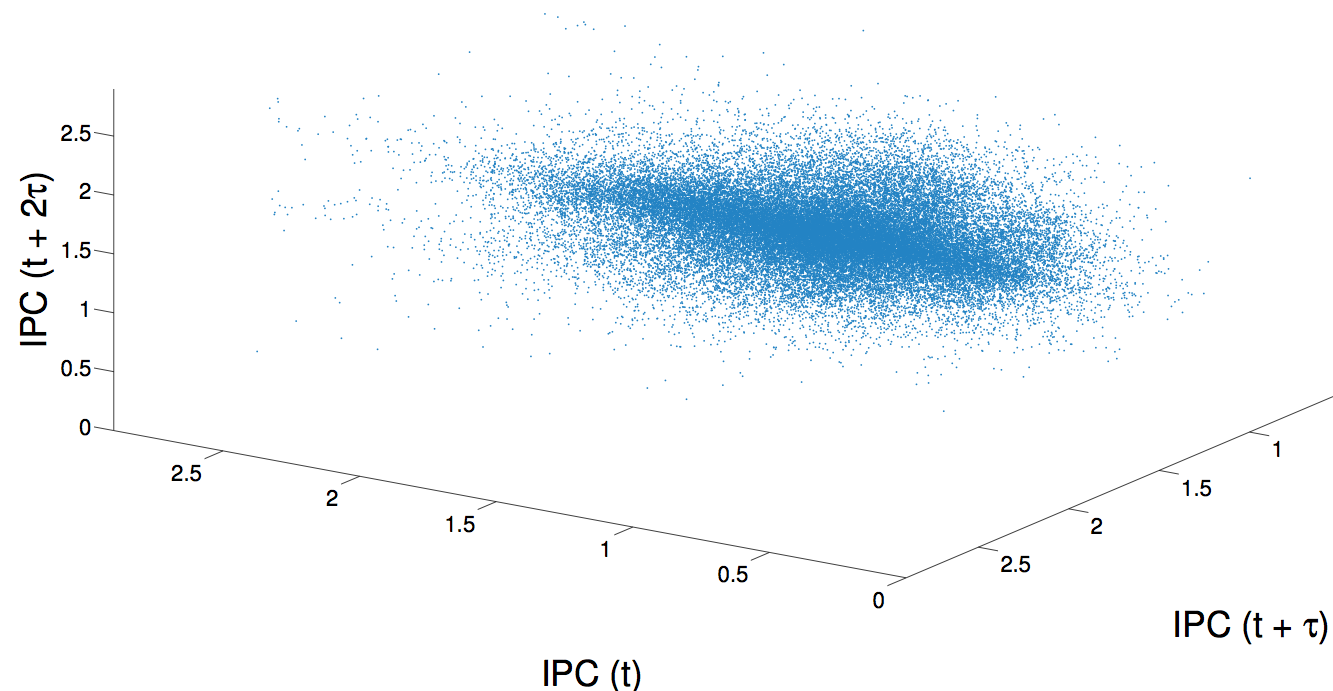
\includegraphics[width=\columnwidth]{figs/gcc3dipc}
    \caption{\gcc}
    \label{fig:gccEmbedding}
  \end{subfigure}
  \\
  \begin{subfigure}{\columnwidth}
    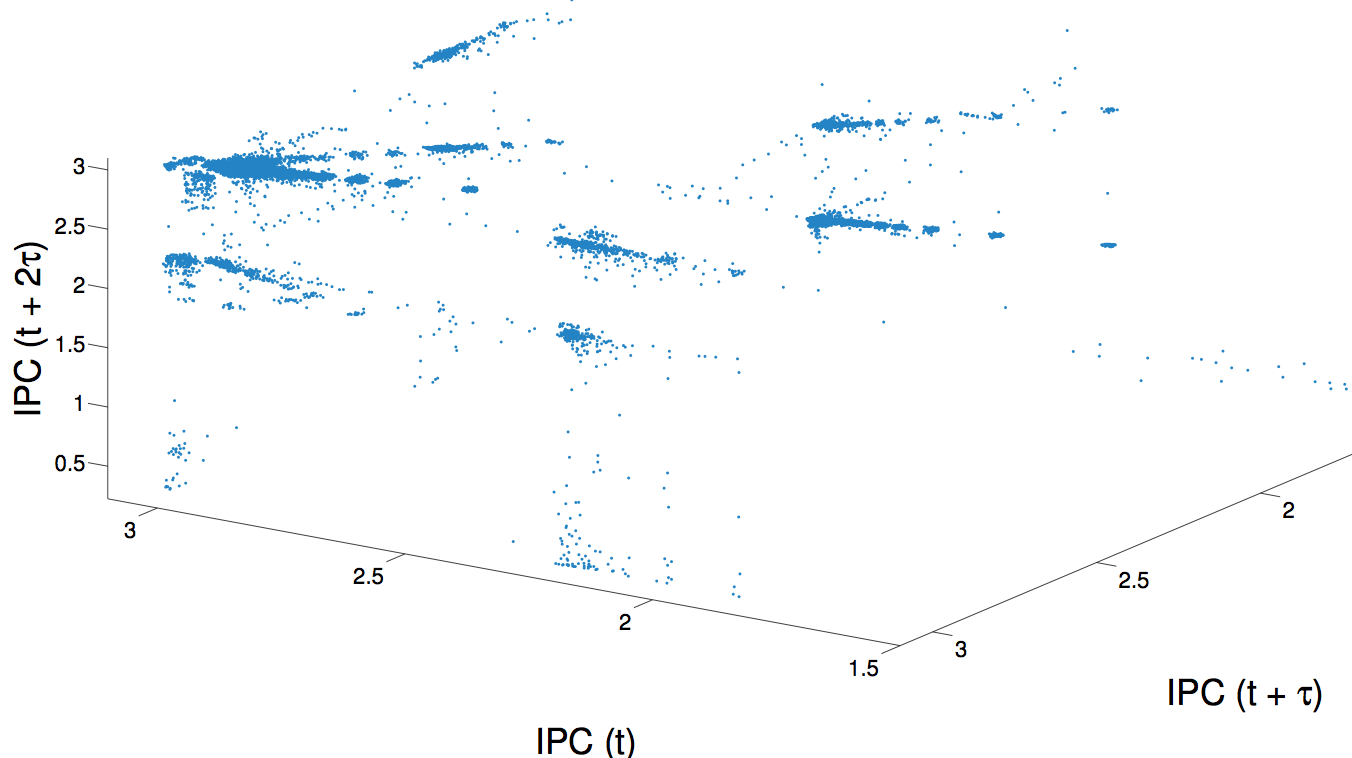
\includegraphics[width=\columnwidth]{figs/svd53dipc2}
    \caption{\svdfive}
    \label{fig:svdfiveEmbedding}
  \end{subfigure}%
%


     %\includegraphics[width=\textwidth]{colipc3d}
     \caption{3D projections of delay-coordinate embeddings of the
       traces from (a) Figure~\ref{fig:col-ts} (b)
       Figure~\ref{fig:gcc-ts} and (c) the fifth (green) segment of
       Figure~\ref{fig:svd-ts-colored}.}
 \label{fig:embedding}
 \end{figure}
%% can cut for space if need be:
%The coordinates of each point in these plots are differently delayed
%elements of the instructions per cycle time series $X_{i,obs}$: that
%is, $X_{i,obs}$ on the first axis, $X_{i+\tau,obs}$ on the second,
%$X_{i+2\tau,obs}$ on the third, and so on.
%

Geometric structure in these kinds of plots is an indication of
structure in the information generation/transmission process that
produced the time series.  The dynamical systems community has
developed a number of methods that leverage this structure to generate
predictions (e.g.,~\cite{weigend-book,casdagli-eubank92,Smith199250}).
One of the most straightforward of these is the \emph{Lorenz method of
  analogues} (LMA), which is essentially nearest-neighbor prediction
in the embedded\footnote{Lorenz's original formulation used the full
  system state space;
%
%According to \cite{kantz97},
%
this method was first extended to embedded dynamics by
Pikovsky~\cite{pikovsky86-sov}, but is also related to the prediction
work of Sugihara \& May~\cite{sugihara90}}
space~\cite{lorenz-analogues}.  Even this simple algorithm---which
builds predictions by finding the nearest neighbor in the embedded
space of the given point, then taking that neighbor's path as the
prediction---provides accurate forecasts when the generating process
is a deterministic dynamical system.

Since LMA does not rest on an assumption of linearity (as ARIMA does),
it can handle both linear and nonlinear processes.  If the underlying
generating process is nondeterministic, however, it can perform
poorly.  In Figure~\ref{fig:embedding}b, for instance, little
structure is visible, so LMA may not work well.  More structure
appears to be present in~Figure~\ref{fig:embedding}c, but this
reconstruction also appears to contain some noise.  The question as to
how much structure is present in a reconstruction---and how much of
that structure can be captured and used by LMA---is apropos of the
central question treated in this paper.  It may be that \gcc has some
redundancy that LMA cannot exploit, or that the structure in \svdfive
is effectively obfuscated, from the standpoint of the LMA method, by
noise.  Without any knowledge of the generating process, answers to
these questions can only be derived from the data, with all of the
attendant problems (noise, sampling issues, etc.)  By quantifying the
balance between redundancy (that is, predictive structure) and entropy
for these real-valued time series, as shown in
Section~\ref{sec:results}, we can begin to answer these questions
in an effective and practical manner.

% If enough predictive structure is present in these embeddings, that
% structure can be used to build an effective forecast model.

\subsection{Assessing Prediction Accuracy}
\label{sec:accuracy}

To study the relationship between predictability and complexity, we
use the four methods outlined above to generate predictions of all 360
traces described in Section~\ref{sec:methods}, then calculate the
error of the predictions with respect to the true continuations.
Specifically, we split each time series into two pieces: the first
90\%, referred to as the ``initial training" signal and denoted
$\{x_i\}_{i=1}^{n}$, and the last 10\%, known as the ``test" signal
$\{c_j\}_{j=n+1}^{k+n+1}$.  The initial training signal is used to
build the model, following the procedures described in the previous
section; that model is used to generate a prediction of the value of
$x_{n+1}$, which is then compared to the true continuation, $c_{n+1}$.
The model is then rebuilt using $\{x_i\}_{i=1}^{n+1}$ and the process
repeats $k$ times, out to the end of the observed time series.  This
``one step prediction'' process is not technically necessary in the
LMA method, whose ability to generate accurate predictions is limited
only by the positive Lyapunov exponents of the system.  However, the
performance of the other three methods used here will degrade severely
if the associated models are not periodically rebuilt.  In order to
make the comparison fair, we used an iterative one-step prediction
schema \emph{for all four methods}.  This has the slightly confusing
effect of causing the ``test'' signal to be used both to assess the
accuracy of each model and for periodic refitting.

Figure~\ref{fig:forecast-example} shows example forecasts made using
all four methods for the \col, \gcc, and \svdfive time series.
\begin{figure*}[htbp]
  \centering

  \begin{subfigure}{0.6\columnwidth}
    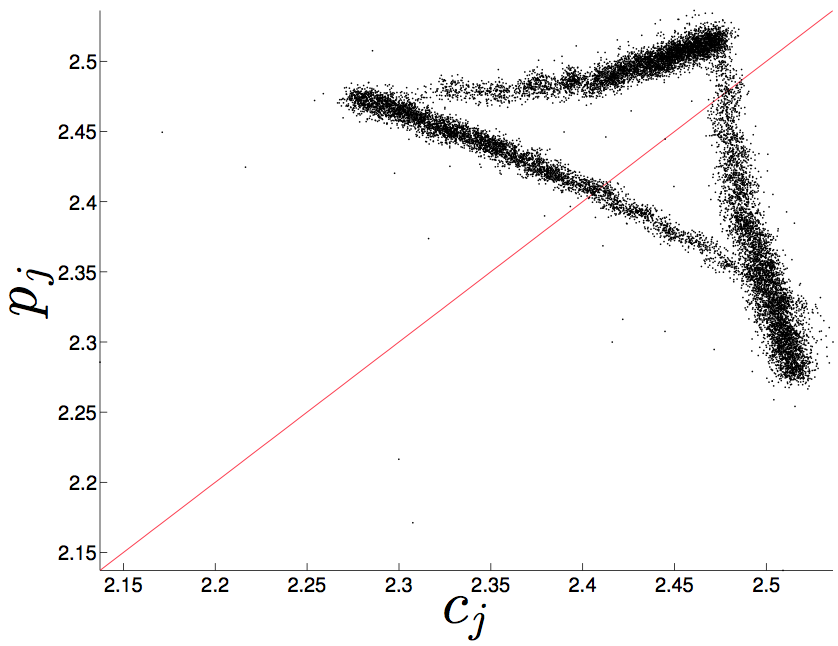
\includegraphics[width=\columnwidth]{figs/colRWForecast}
    \caption{\col\\ random walk }
    \label{fig:colRW}
  \end{subfigure}%
   \begin{subfigure}{0.6\columnwidth}
    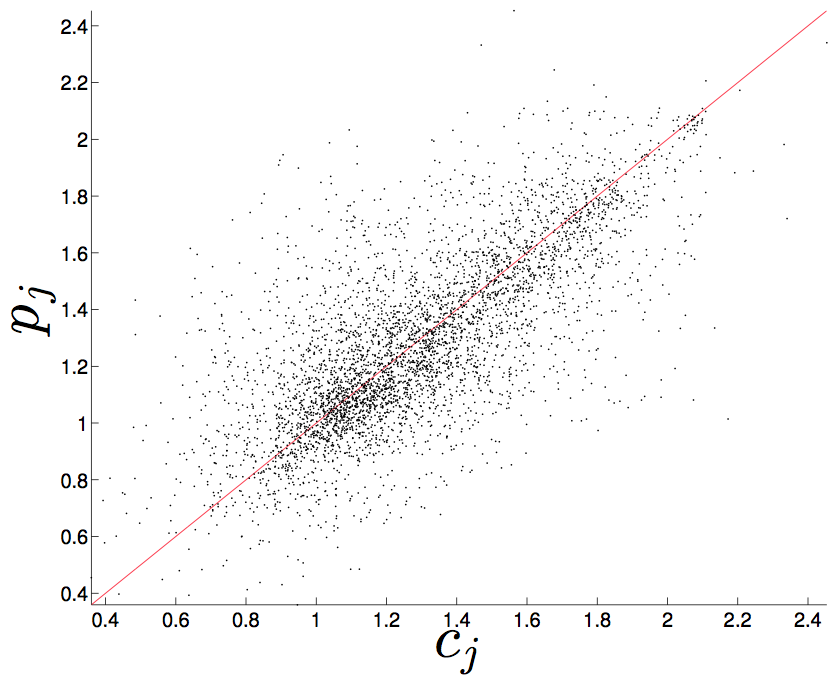
\includegraphics[width=\columnwidth]{figs/gccRWForecast}
    \caption{\gcc\\ random walk }
    \label{fig:gccRW}
  \end{subfigure}%
     \begin{subfigure}{0.6\columnwidth}
    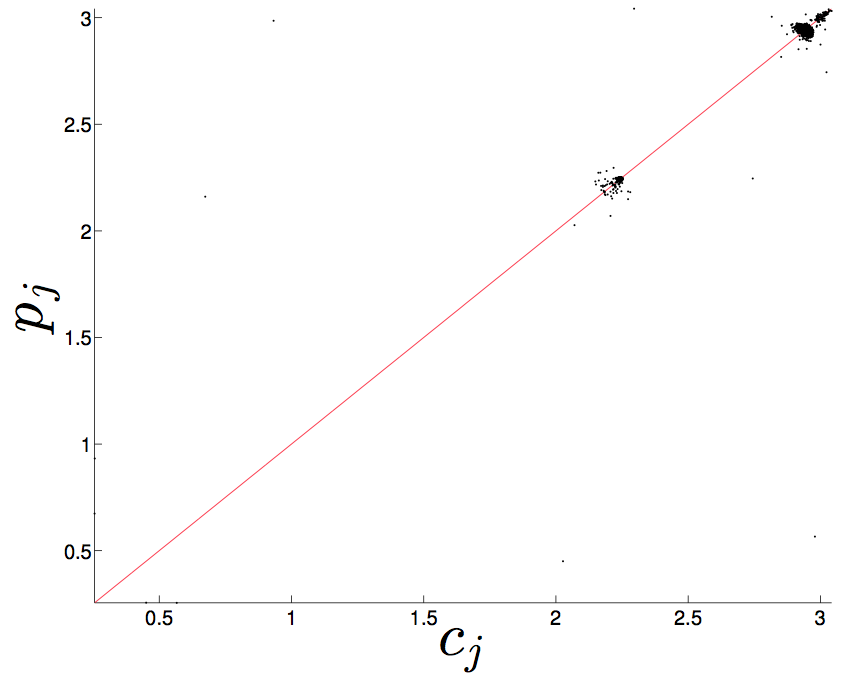
\includegraphics[width=\columnwidth]{figs/svdfiveRWForecast}
    \caption{\svdfive\\ random walk}
    \label{fig:svd5RW}
  \end{subfigure}%
  \\
      \begin{subfigure}{0.6\columnwidth}
    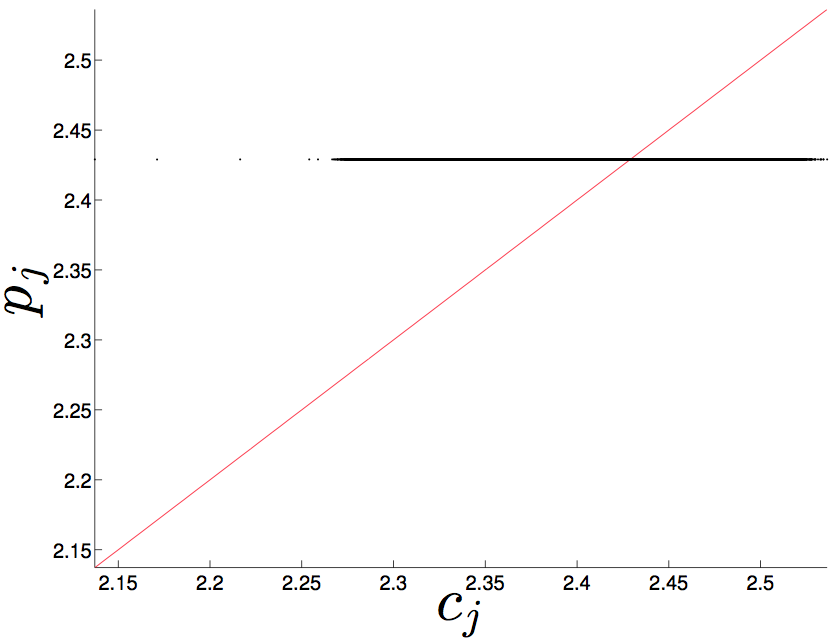
\includegraphics[width=\columnwidth]{figs/colMeanForecast}
    \caption{\col\\ na\"ive }
    \label{fig:colMEAN}
  \end{subfigure}%
   \begin{subfigure}{0.6\columnwidth}
    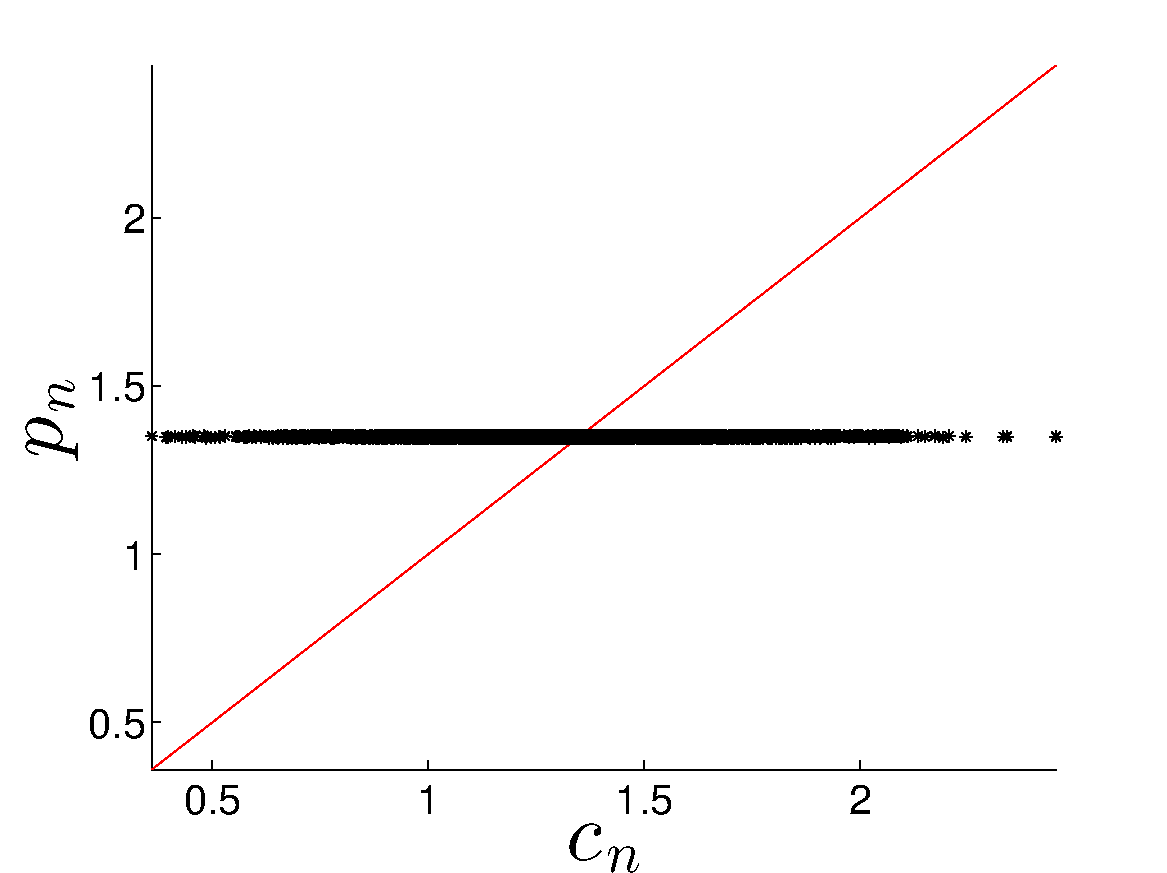
\includegraphics[width=\columnwidth]{figs/gccMeanForecast}
    \caption{\gcc\\ na\"ive }
    \label{fig:gccMEAN}
  \end{subfigure}%
     \begin{subfigure}{0.6\columnwidth}
    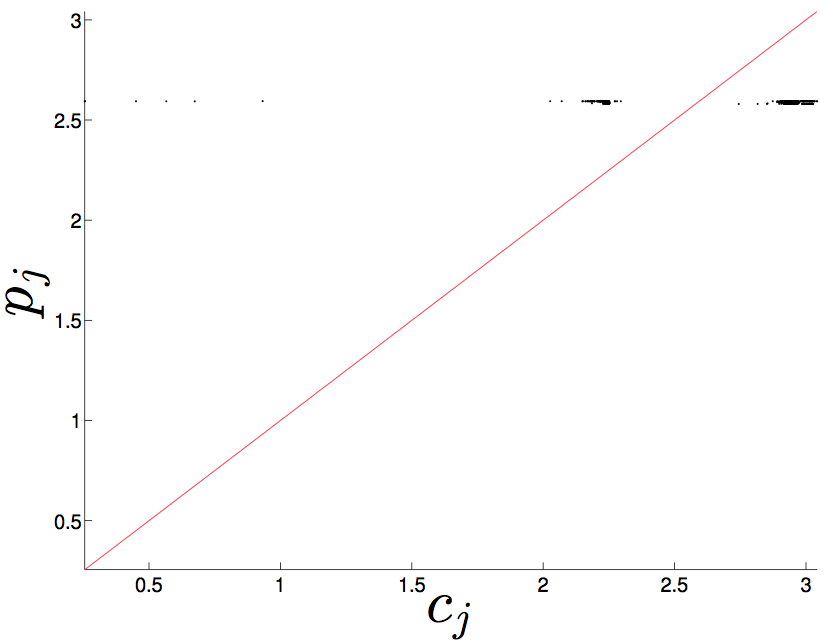
\includegraphics[width=\columnwidth]{figs/svdfiveMeanForecast}
    \caption{\svdfive\\ na\"ive }
    \label{fig:svd5MEAN}
  \end{subfigure}%
  \\
    \begin{subfigure}{0.6\columnwidth}
    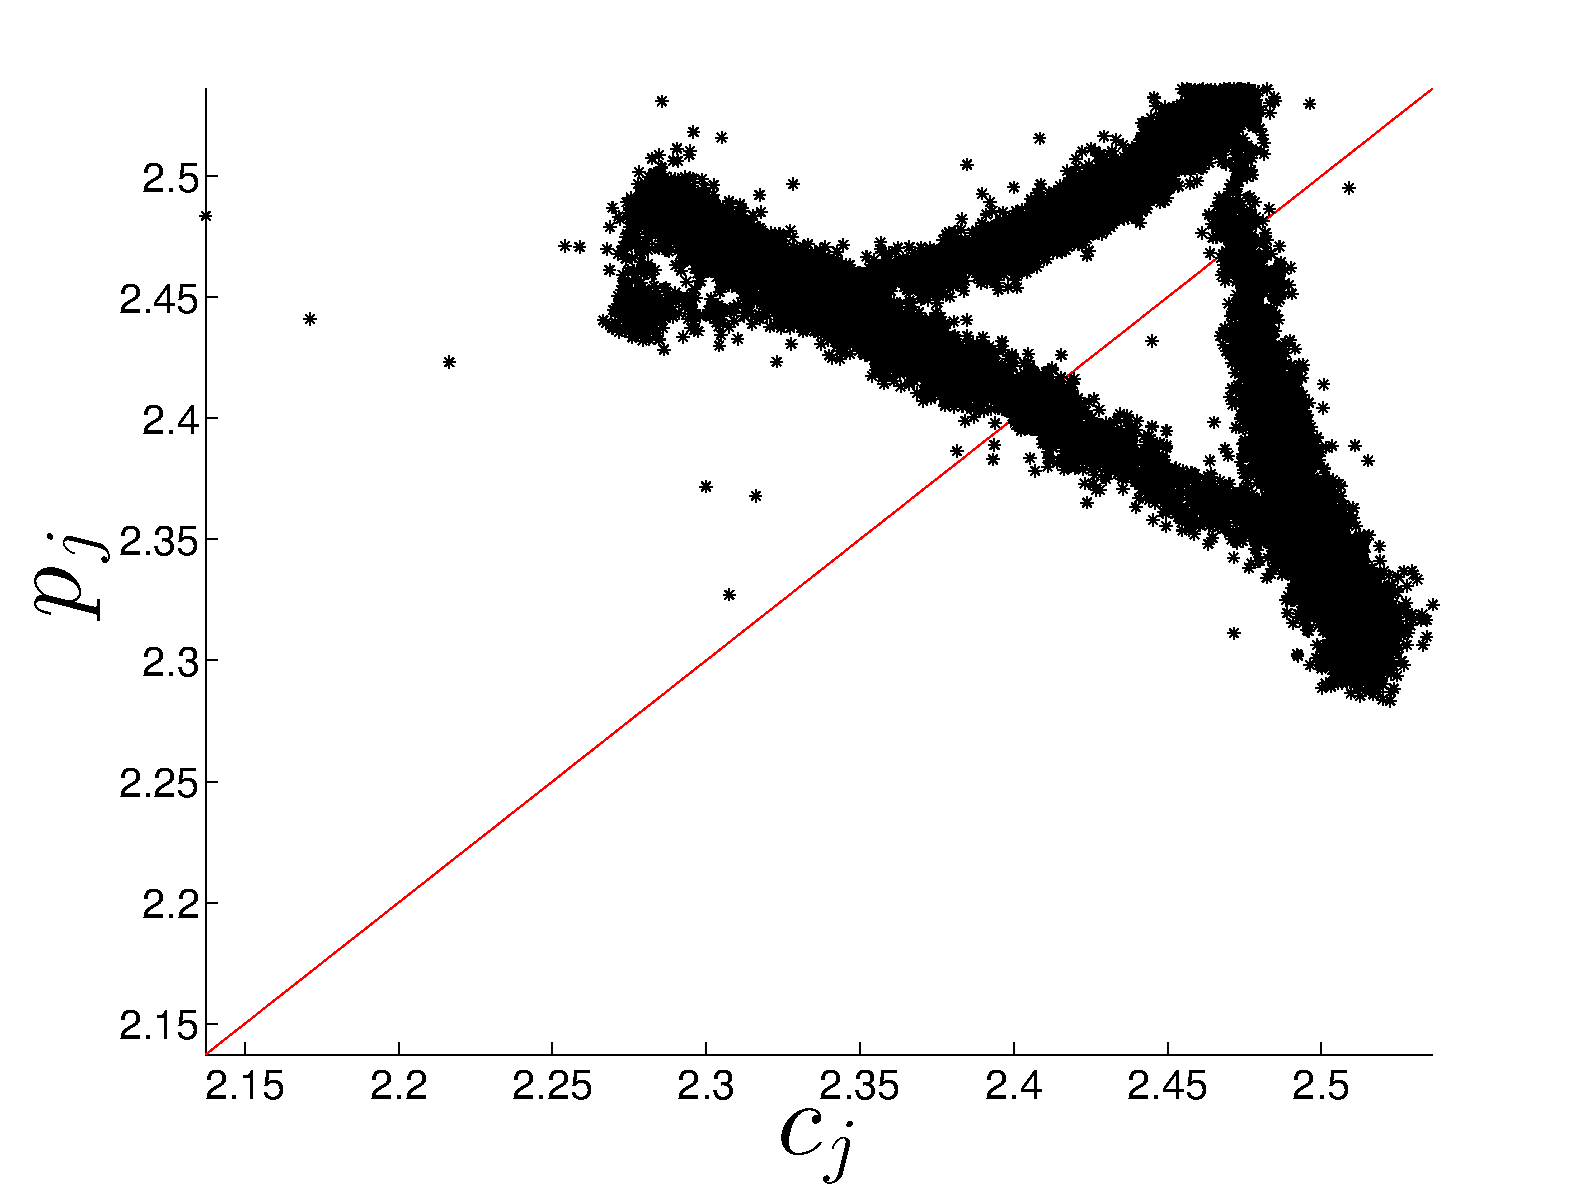
\includegraphics[width=\columnwidth]{figs/colARIMAForecast}
    \caption{\col \\ ARIMA}
    \label{fig:colARIMA}
  \end{subfigure}
  \begin{subfigure}{0.6\columnwidth}
    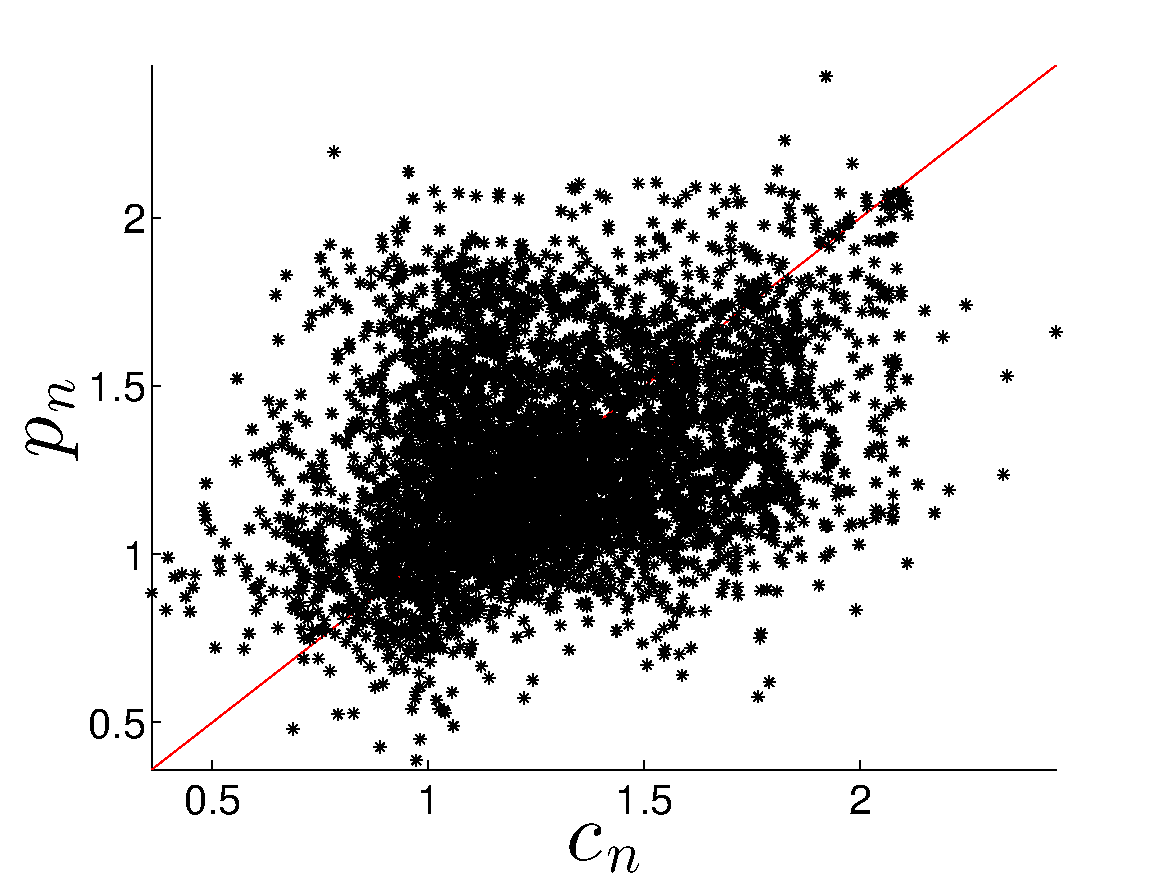
\includegraphics[width=\columnwidth]{figs/gccARIMAForecast}
    \caption{\gcc \\ ARIMA }
    \label{fig:gccARIMA}
  \end{subfigure}%
  \begin{subfigure}{0.6\columnwidth}
    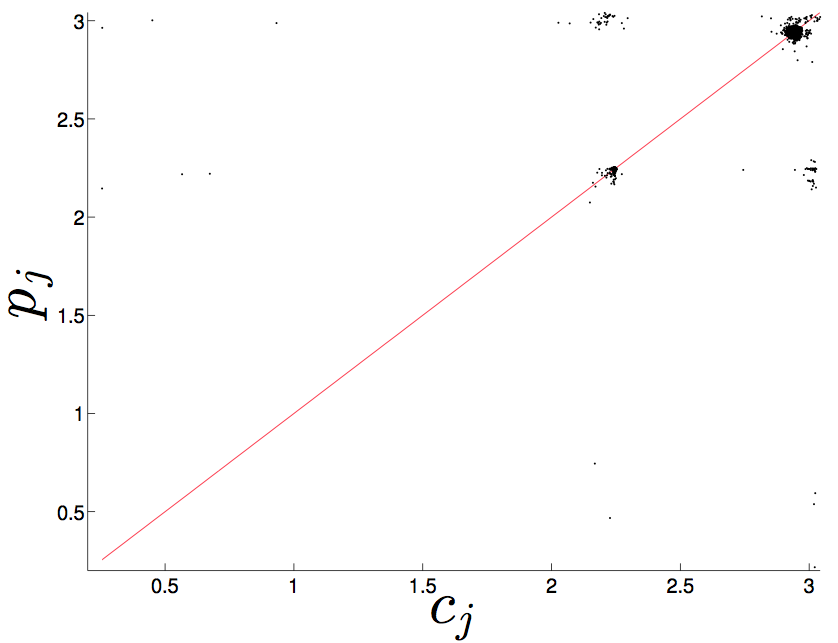
\includegraphics[width=\columnwidth]{figs/svdfiveARIMAForecast}
    \caption{\svdfive \\ ARIMA }
    \label{fig:svd5ARIMA}
  \end{subfigure}%
  \\

      \begin{subfigure}{0.6\columnwidth}
    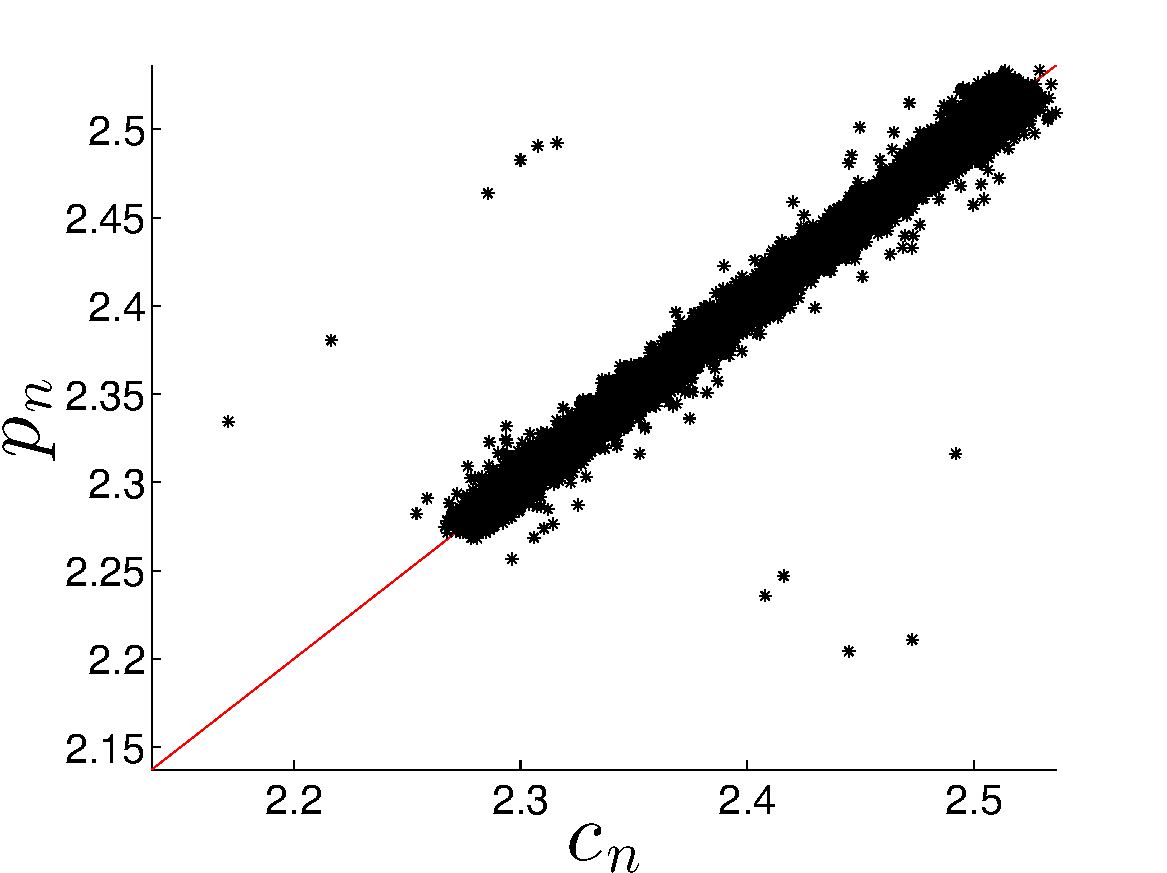
\includegraphics[width=\columnwidth]{figs/colLMAForecast}
    \caption{\col \\ LMA}
    \label{fig:colLMA}
  \end{subfigure}
      \begin{subfigure}{0.6\columnwidth}
    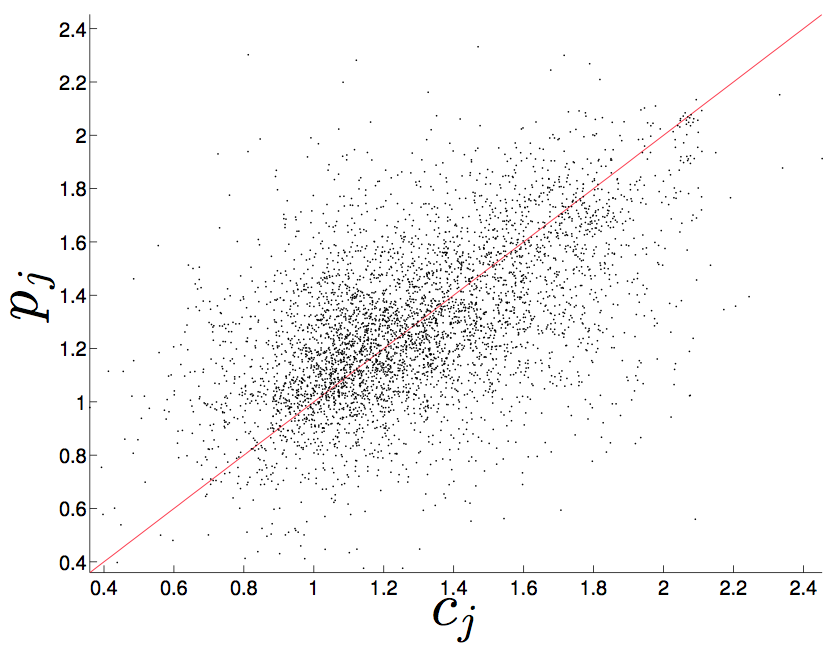
\includegraphics[width=\columnwidth]{figs/gccLMAForecast}
    \caption{\gcc \\ LMA}
    \label{fig:gccLMA}
  \end{subfigure}
        \begin{subfigure}{0.6\columnwidth}
    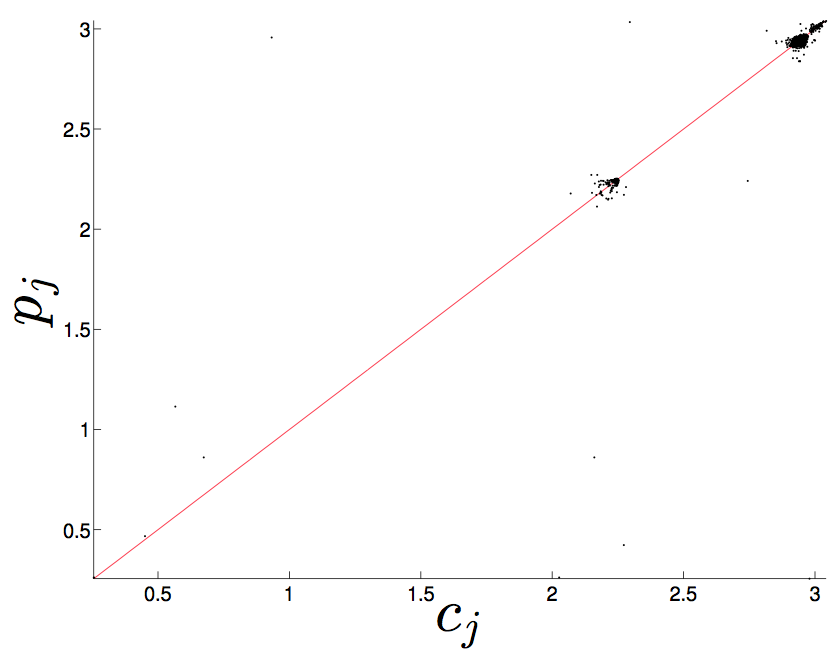
\includegraphics[width=\columnwidth]{figs/svdfiveLMAForecast}
    \caption{\svdfive \\ LMA}
    \label{fig:svd5LMA}
  \end{subfigure}
  %\begin{subfigure}{0.5\textwidth}
  %  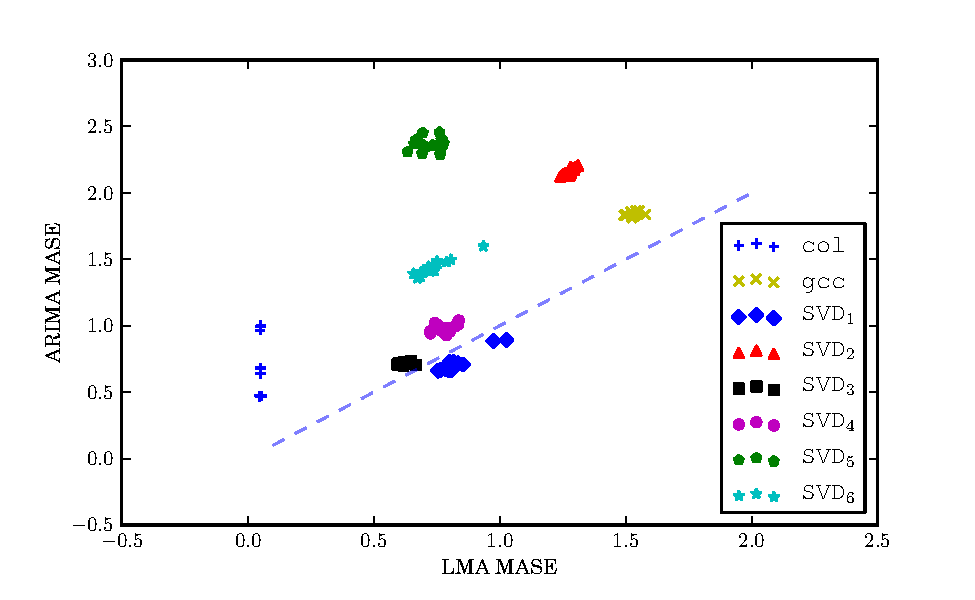
\includegraphics[width=1.0\textwidth]{LMA_vs_ARIMA}
   \caption{Predicted ($p_j$) versus true values ($c_j$) for
     forecasts of \col, \gcc, and \svdfive and all four prediction strategies.
% On this type of plot, a perfect prediction lies exactly on the
% diagonal.
%
%
}
\label{fig:forecast-example}
  %\end{subfigure}
\end{figure*}

\begin{table*}
  \renewcommand{\arraystretch}{1.25}
  \begin{tabular}{lccc}
    & {\large \col} & {\large \gcc} & {\large \svdfive} \\
    & & & \\
    \begin{sideways}\large random walk\end{sideways} &
    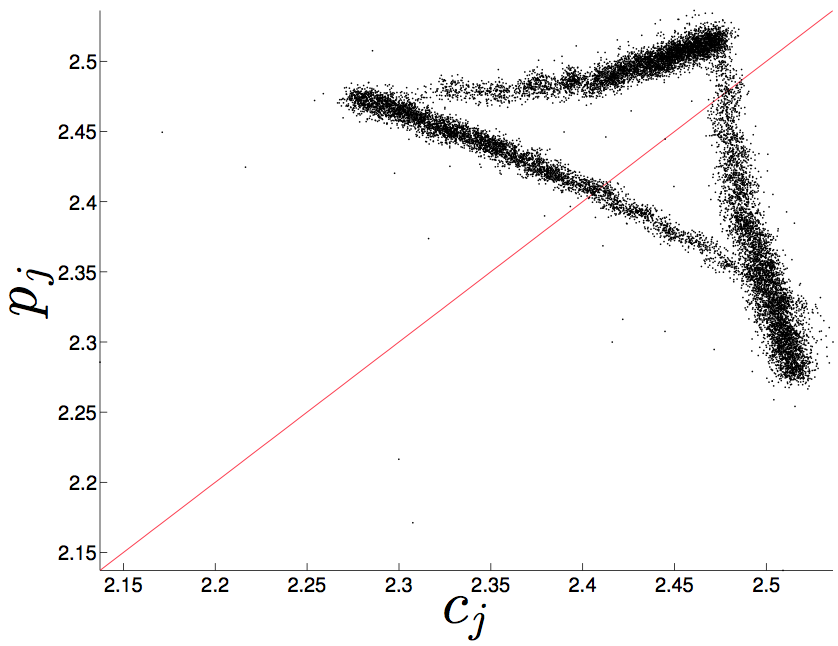
\includegraphics[width=0.6\columnwidth]{figs/colRWForecast} &
    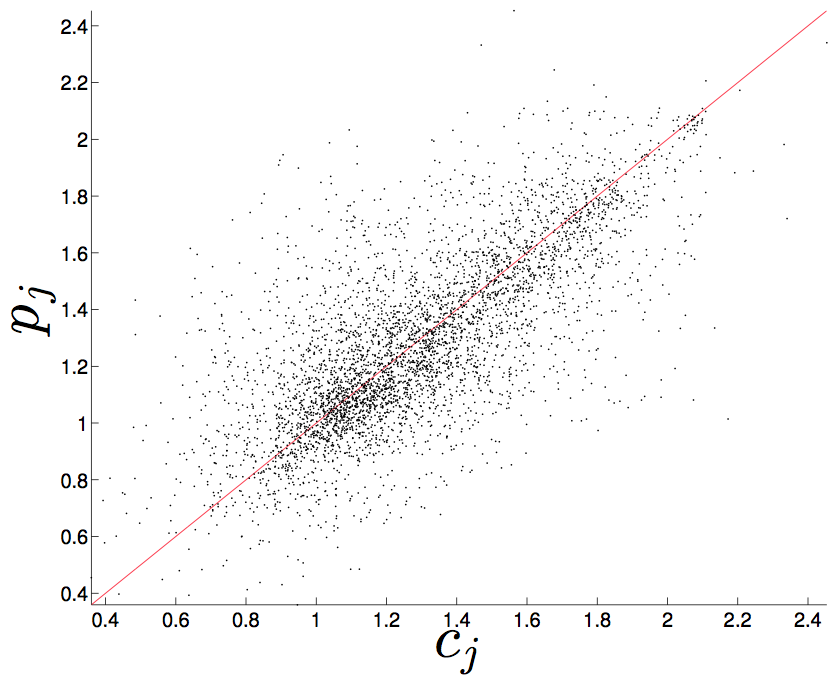
\includegraphics[width=0.6\columnwidth]{figs/gccRWForecast} &
    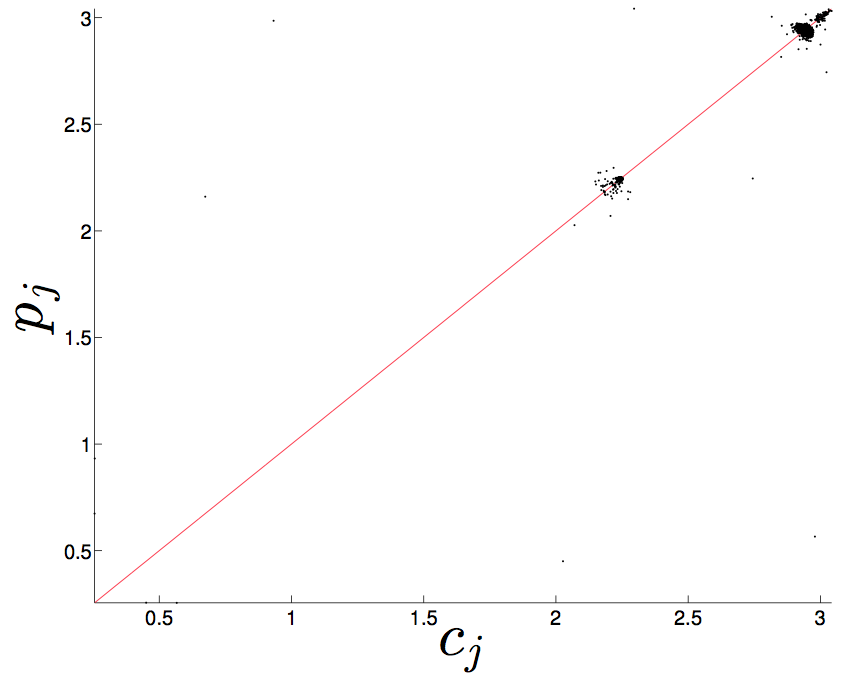
\includegraphics[width=0.6\columnwidth]{figs/svdfiveRWForecast} \\
    \begin{sideways}\large na\"ive\end{sideways} &
    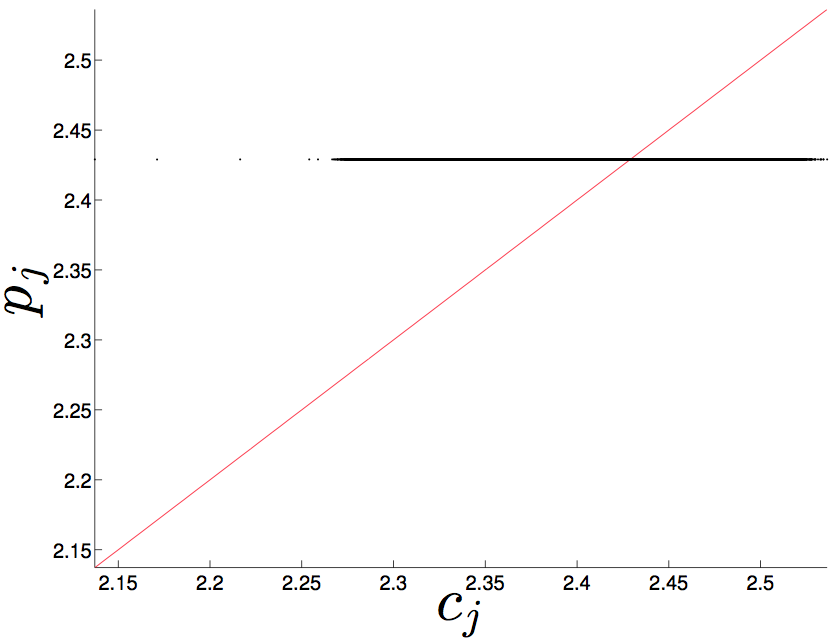
\includegraphics[width=0.6\columnwidth]{figs/colMeanForecast} &
    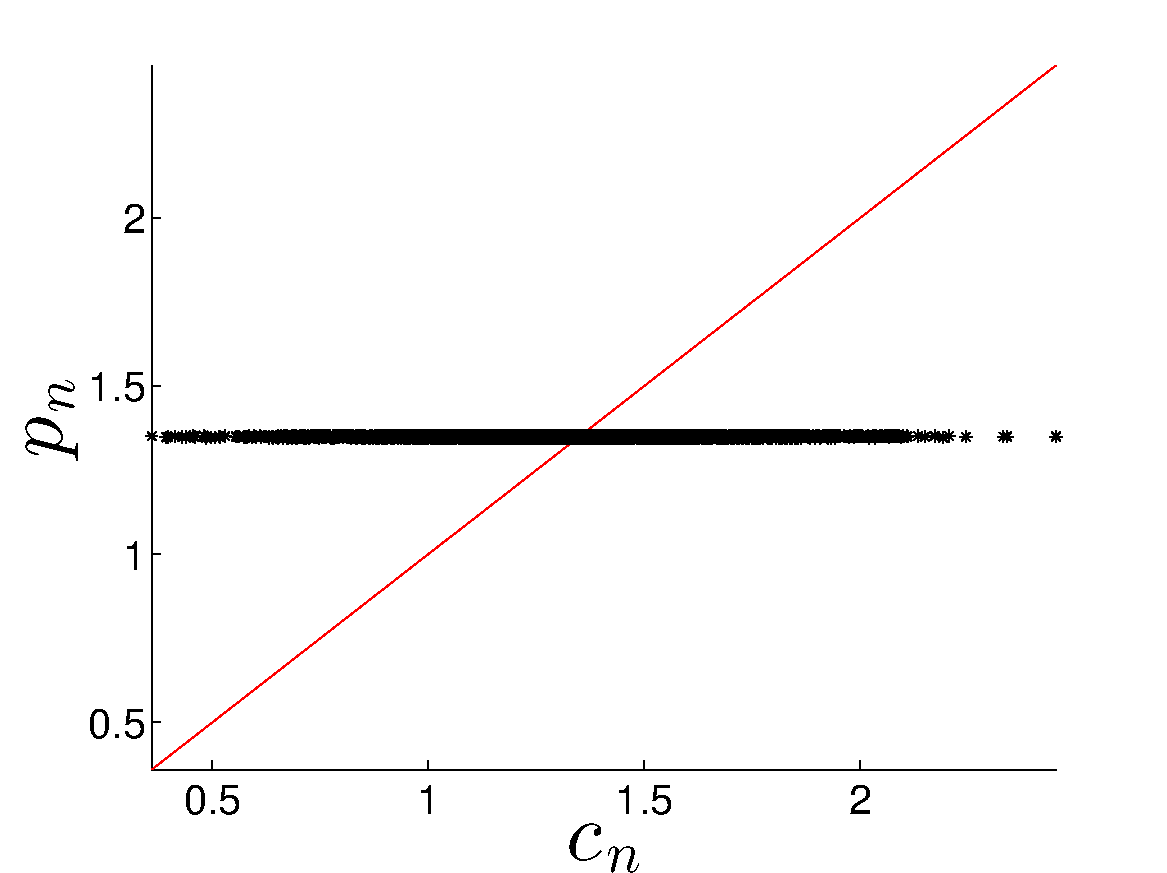
\includegraphics[width=0.6\columnwidth]{figs/gccMeanForecast} &
    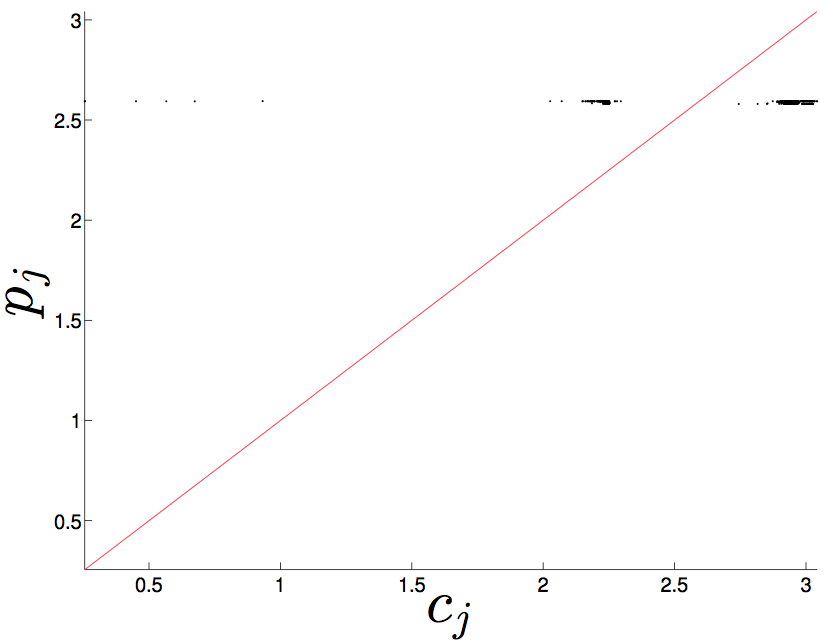
\includegraphics[width=0.6\columnwidth]{figs/svdfiveMeanForecast} \\
    \begin{sideways}\large ARIMA\end{sideways} &
    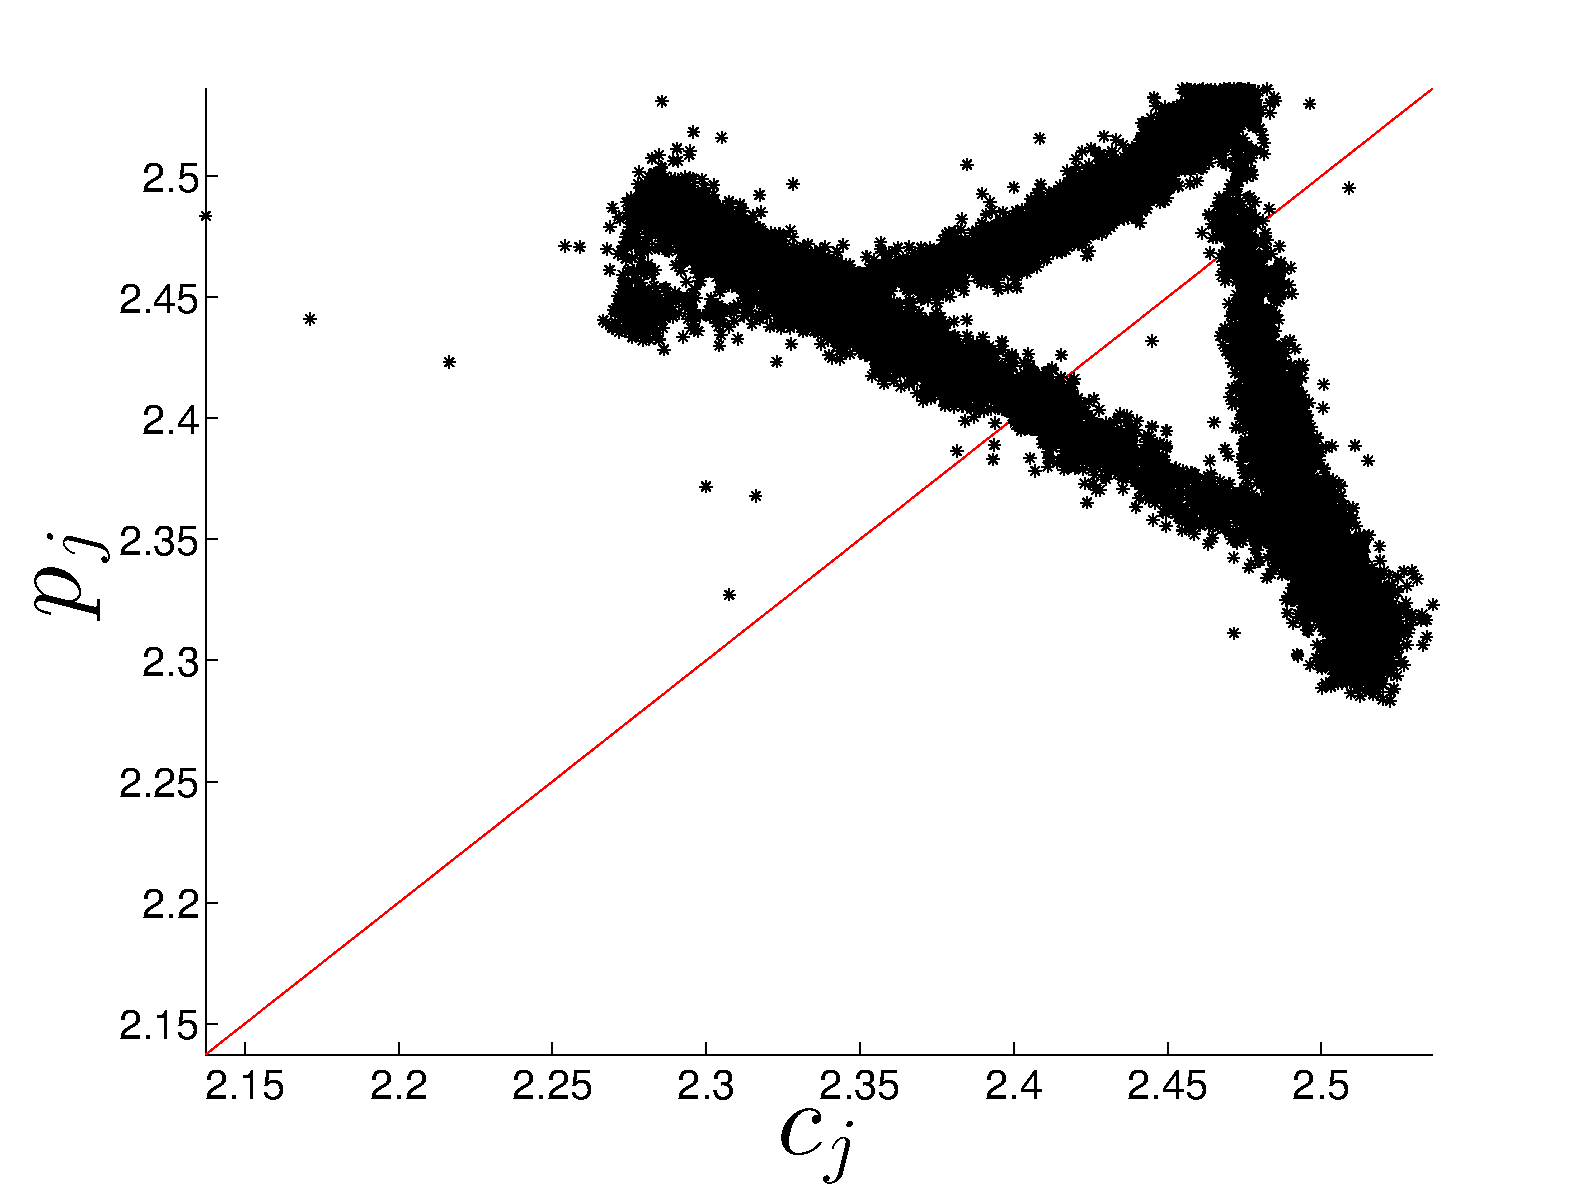
\includegraphics[width=0.6\columnwidth]{figs/colARIMAForecast} &
    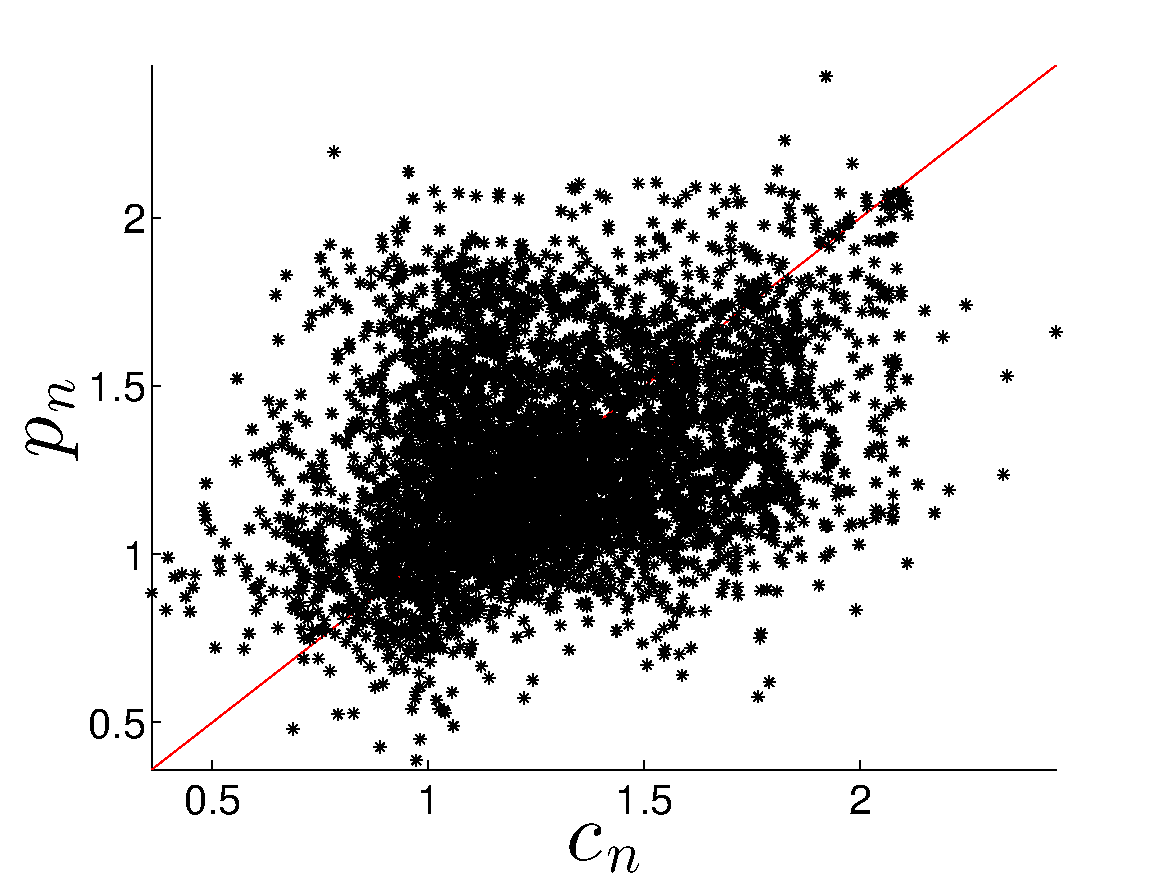
\includegraphics[width=0.6\columnwidth]{figs/gccARIMAForecast} &
    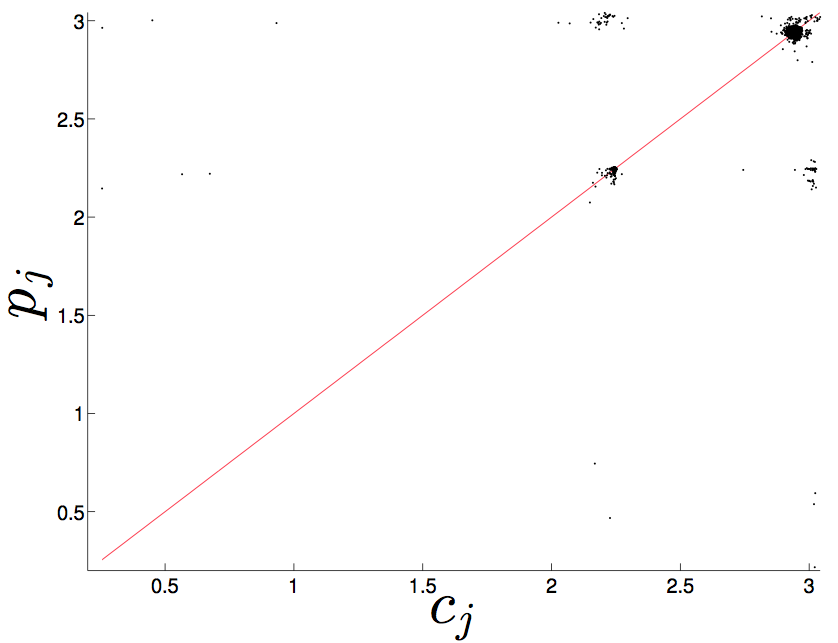
\includegraphics[width=0.6\columnwidth]{figs/svdfiveARIMAForecast} \\
    \begin{sideways}\large LMA\end{sideways} &
    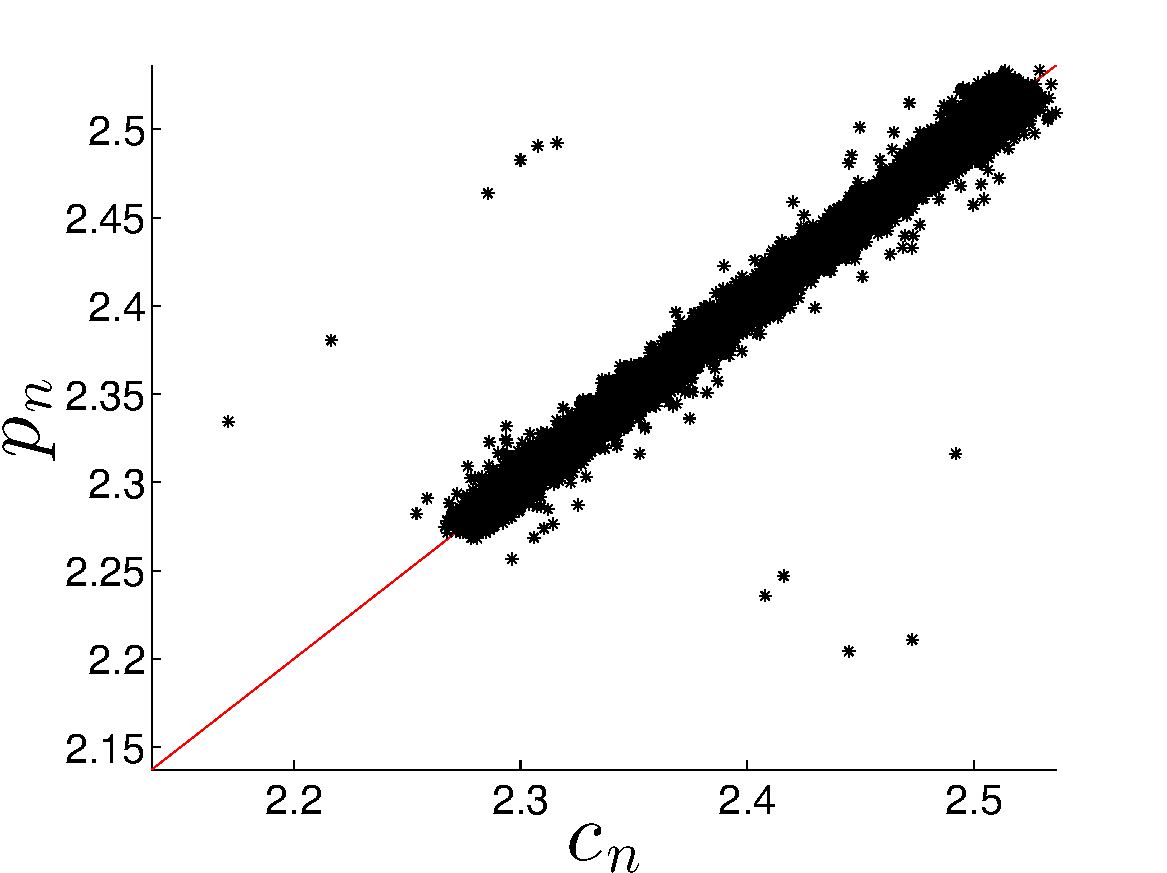
\includegraphics[width=0.6\columnwidth]{figs/colLMAForecast} &
    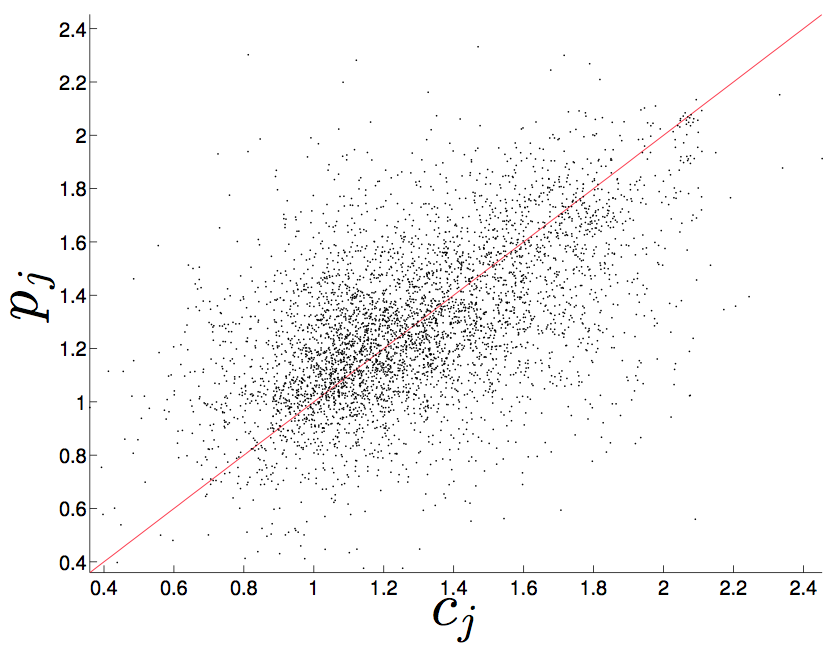
\includegraphics[width=0.6\columnwidth]{figs/gccLMAForecast} &
    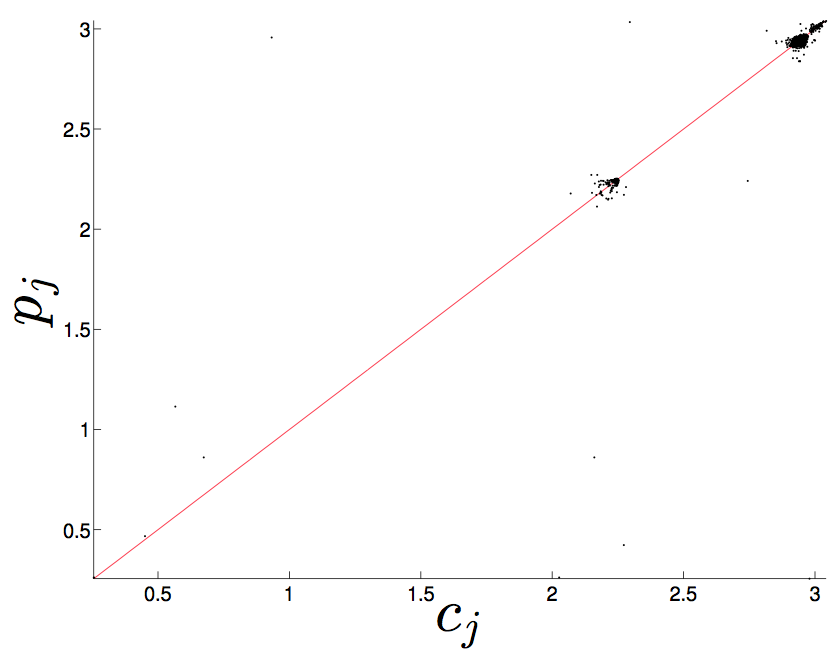
\includegraphics[width=0.6\columnwidth]{figs/svdfiveLMAForecast}
  \label{fig:forecast-example}
  \end{tabular}
  \caption{Predicted ($p_j$) versus true values ($c_j$) for forecasts of \col,
     \gcc, and \svdfive and all four prediction strategies.
  }
  \label{fig:forecast-example}
\end{table*}
In these images, the vertical axis is the prediction $p_j$ and the
horizontal axis is the true continuation $c_j$.  On such a plot, a
perfect prediction would lie on the diagonal.  LMA, for instance,
generates a very accurate prediction of the \col data, while ARIMA
does not.  Horizontal lines result when a constant predictor (e.g.,
\naive) is used on a non-constant signal.  Point clouds reflect the
structure of the distribution of the errors---roughly normally
distributed, for example, in the case of LMA on \gcc.  Note that the
shapes of Figures~\ref{fig:colRW} and~\ref{fig:colARIMA} are
reminiscent of the projected embedding in Figure~\ref{fig:embedding}a.
For a random-walk predictor, a $p_j$ vs. $c_j$ plot is equivalent to a
two-dimensional embedding with $\tau=1$.  For ARIMA, the
correspondence is not quite as simple, since the $p_j$ values are
linear combinations of a number of past values of the $c_j$, but the
effect is largely the same\footnote{The temporal \emph{ordering} of
  the points on the ARIMA $p_j$ vs. $c_j$ plot does not match that of
  a projected embedding of the time series, however.}.

As a numerical measure of prediction accurary, we calculate the mean
absolute scaled error (MASE) between the true and predicted signals:
%
$$MASE = \sum_{j=n+1}^{k+n+1}\frac{|p_j-c_j|
}{\frac{k}{n-1}\sum^n_{i=2}|x_{i}-x_{i-1}|}$$
%
This error metric was introduced in \cite{MASE} as a ``generally
applicable measurement of forecast accuracy without the problems seen
in the other measurements."  MASE is a normalized measure: the scaling
term in the denominator
%
% of the MASE value
% $$\frac{1}{n-1}\sum^n_{i=2}|X_{i,obs}-X_{i-1,obs}|$$
%
is the average in-sample forecast error for a random-walk prediction
over the initial training signal $\{x_i\}^n_{i=1}$.  That is, $MASE<1$ means that the
prediction error in question was, on the average, smaller than the
error of a random-walk forecast on the same data.  Analogously,
$MASE>1$ means that the corresponding prediction method did
\emph{worse}, on average, than the random-walk method.  We chose this
error metric because it allows for fair comparison across varying
methods, prediction horizons, and signal scales.

MASE scores for all 360 experiments are tabulated in the three
middle columns in Table~\ref{tab:error}.
\begin{table*}
\caption{Mean
absolute scaled error (MASE) scores and weighted permutation entropies for all eight
   processes studied in this paper}
  \begin{center}
  \begin{tabular*}{\textwidth}{@{\extracolsep{\fill} } ccccc}
  \hline\hline Signal & LMA MASE  & ARIMA MASE & na\"{i}ve MASE  & Weighted Permutation Entropy \\
  \hline
 \col           & $ 0.050 \pm0.002  $ & $0.599  \pm 0.211 $ & $0.571\pm0.002$&  $0.513 \pm 0.003$ \\

\gcc           & $ 1.530\pm 0.021$ & $1.837 \pm0.016 $ & $0.951 \pm 0.001$ & $0.943 \pm 0.001$ \\

\svdone     & $ 0.827\pm 0.076$ & $ 0.714\pm 0.075 $ & $2.676\pm4.328$&  $0.957 \pm 0.016$ \\

 \svdtwo    & $1.279 \pm0.020 $ & $2.163 \pm0.027 $ &  $3.054\pm0.040$ &   $0.846 \pm0.004$ \\

\svdthree     & $0.619 \pm0.021 $ & $0.713 \pm 0.010 $ & $31.386\pm 0.282$ &  $0.716 \pm 0.006$ \\
 \svdfour     & $ 0.779\pm0.036 $ & $0.979 \pm0.032 $ & $2.661\pm0.074$ & $0.825 \pm 0.008$ \\

\svdfive     & $ 0.718\pm 0.048 $ & $2.370  \pm 0.051 $ & $20.870 \pm 0.192$&  $0.678 \pm 0.007$ \\
 \svdsix     & $ 0.739\pm 0.068 $ & $ 1.438\pm 0.061$ & $2.197\pm0.083$&  $0.748 \pm 0.011$ \\
  \hline\hline
  \end{tabular*}
  \end{center}
 \label{default}
 \label{tab:error}
  \end{table*}%
Comparing these with the geometry of the plots in
Figure~\ref{fig:forecast-example}, one can see some obvious
correspondences.  The average LMA MASE score for the \col signals
was $0.050$, for instance, while ARIMA scored much worse ($0.599$).
That is, LMA performed roughly 20 times better on \col signals than a
random-walk predictor, while ARIMA only outperformed random walk by a
factor of 1.7.  This is in accordance with the visual appearance of
the corresponding images in Figure~\ref{fig:forecast-example}.  While
the correspondence between MASE score and the visual appearance of
these kinds of plots is clear cut in this case, that is not always so.
The plots of LMA predictions of \col and \svdfive both lie near the
diagonal, for instance, but the corresponding MASE scores were very
different: $0.050$ for \col and $0.718$ for \svdfive (resp., 20 and
1.4 times better than random-walk forecasts of the same signals).
This is a result of the normalization in the MASE score calculation.
Recall from Section~\ref{sec:simple} that the random-walk method
performs especially poorly on signals that oscillate rapidly.  \col
fits this description, so the random-walk error on this signal---the
denominator of the three MASE scores in the first row of the
Table---is pathologically high, which skews those scores down.
Random-walk prediction is very effective for the \svdfive signal, on
the other hand, so the denominator is small and the MASE scores are
skewed upwards.  Normalization is, as is often the case, a double-edged
sword.  Here, it facilitates comparisons across signals of different
types and lengths, but its particular pathologies must be taken into
account, as discussed at more length in Section~\ref{sec:results}.

% Table \ref{tab:error} provides the MASE distributions
% {\color{red}[[Joshua: Ryan, Is this the right word? we give mean $\pm$
%       std. dev but some have very skewed right tails]]} for each of
% the eight signals and three prediction strategies, these are averaged
% over 15 runs of each signal-method combination. For later comparison,
% Table \ref{tab:error} also has the complexity measure we introduce in
% Section \ref{sec:meaComplex}.

%[[and cherry pick a few examples of \gcc and \col to put in the text ]]


%---works quite well on the trace in Figure~%\ref{fig:ipc}, as%
%shown in Figure~\ref{fig:lmacol}.
%
%\begin{figure}
%   \centering
%\begin{subfigure}{\columnwidth}
%    \includegraphics[width=\columnwidth]{%colPredShortTS}
%    \caption{\col }
%    \label{fig:lmacol}
%  \end{subfigure}%
%
%    \begin{subfigure}{\columnwidth}
%    \includegraphics[width=\columnwidth]{%colPredShortTS}
%    \caption{\gcc}
%    \label{fig:lmagcc}
%  \end{subfigure}
%  \begin{subfigure}{\columnwidth}
%%    \includegraphics[width=\columnwidth]{%colPredShortTS}
%    \caption{\svdfive}
%    \label{fig:lmasvdfive}
%  \end{subfigure}%
%  \caption{{\color{red} [[If Liz thinks we should %include these I actually need to generate this %figure]]}An LMA-based forecast of
%       processor-efficiency performance trace from the%\col ,\gcc and \svdfive generating processes.  Red %circles and blue $\times$s are the true and
%       predicted values, respectively; vertical bars %show where these
%       values differ.}\label{fig:lmapredictions}
% \end{figure}
%
%\begin{figure}[htbp]
%  \centering
%   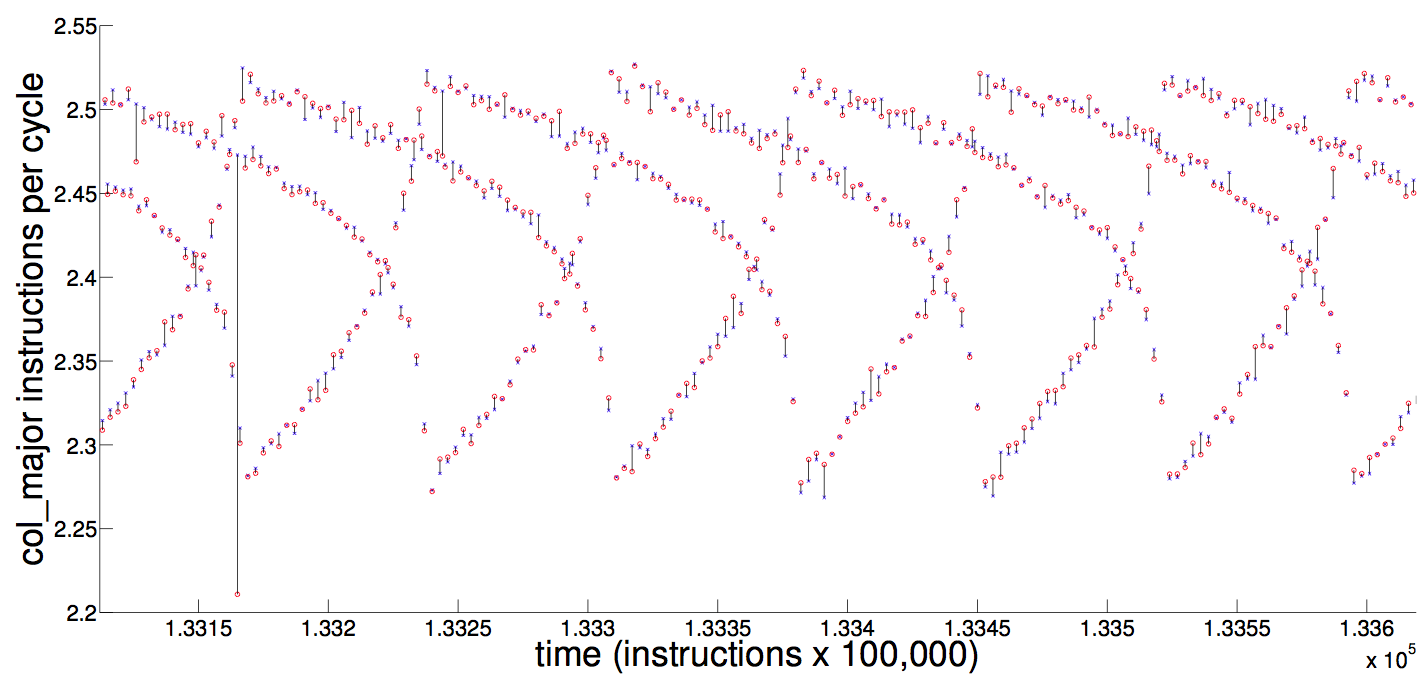
\includegraphics[width=\textwidth]{colPredShortTS}
%    \caption{A forecast of the last 4,000 points of the %signal in
%      Figure~\ref{fig:ipc} using an LMA-based strategy on %the
%      embedding in Figure~\ref{fig:embedding}.  Red circles %and blue
%      $\times$s are the true and predicted values, %respectively;
%      vertical bars show where these values differ.}
%\label{fig:lmacol}
%\end{figure}
%
%\begin{figure}[htbp]
%  \centering
%    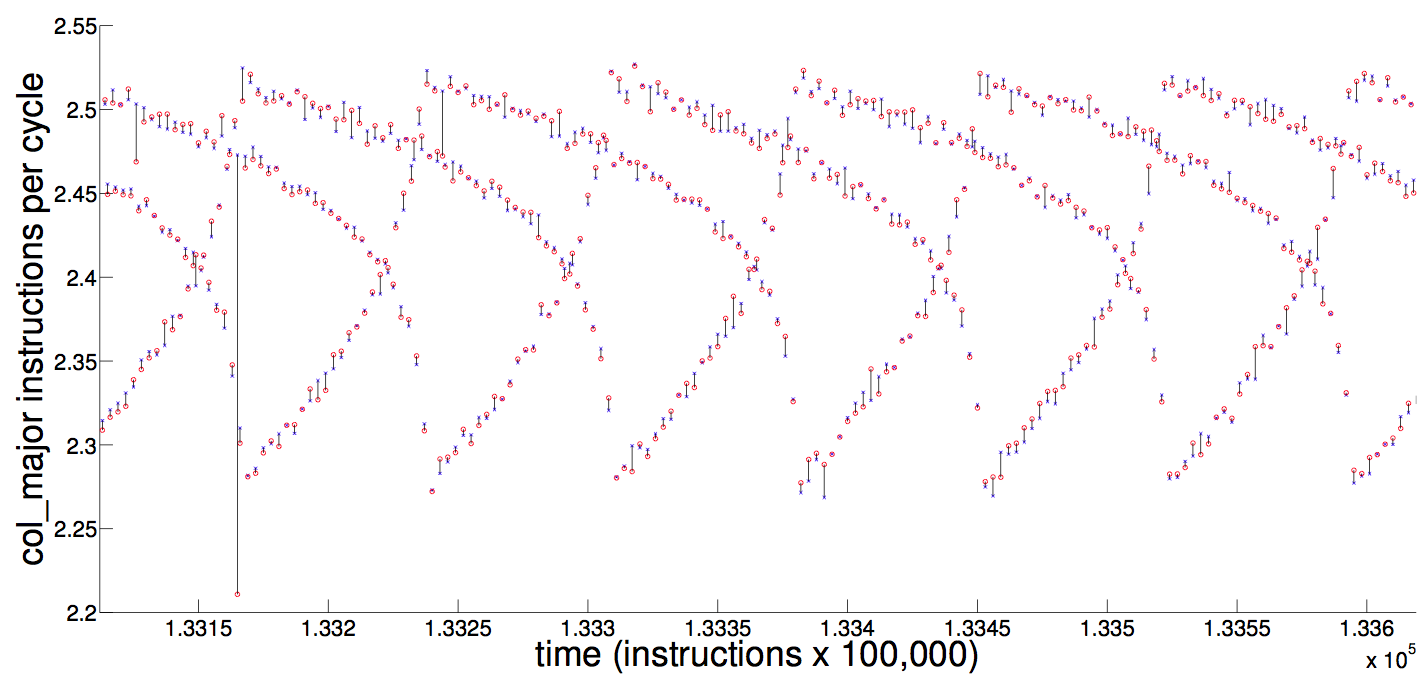
\includegraphics[width=\textwidth]{colPredShortTS}
%     \caption{{\color{red} [[actually need to generate this %figure]]}An LMA-based forecast of the last 4,000 points of a
%       processor-load performance trace from the \gcc
%       benchmark.  Red circles and blue $\times$s are the %true and
%       predicted values, respectively; vertical bars show %where these
%       values differ.}
%\label{fig:lmagcc}
%\end{figure}
%
%On the other hand, if we use the same approach to %forecast the
%processor efficiency (IPC) of the \gcc time series, %the
%prediction is far less accurate; see Figure~%\ref{fig:lmagcc}.
%Figure~\ref{fig:lmasvdfive} is clearly a better %prediction than Figure~\ref{fig:gccLMA} but not nearly as good as the \col forecast.


%This gets at the utility of the contribution of this %paper: These time series all come from the same system---computers---but they are not equally predictable (at this point by LMA). For a practitioner is it the case that
%  Our
%conjecture is that while they come from similar systems \gcc produces processor load traces on the top of the complexity spectrum whereas \col produces processor loads with complexity in the mid to low region of the complexity spectrum. If this is the case then \gcc might be much better predicted using a method like Random Walk or \naive which can effectively predict in the presence of complexity. This is explored more rigorously in the results Section of this paper (Section \ref{sec:results}. So that we don't have to compare the forecast accuarcy by visual comparing the predictions we calculate a figure of merit to compare the predictions.




